\documentclass{article}
\usepackage[utf8]{inputenc}
\usepackage{amsmath}
\usepackage{amsfonts}
\usepackage{graphicx}
\usepackage{amssymb}
\usepackage{amsthm}
\usepackage{float}
\usepackage{tikz}
\usepackage{mlmodern}
\usepackage{subfig}
\usepackage{pgfornament}
\usepackage{graphicx}
\usepackage[some]{background}
\usepackage[T1]{fontenc}
\usepackage[left=2.5cm,right=2.5cm]{geometry}
\usepackage[linesnumbered,ruled]{algorithm2e}
\usepackage{hyperref, xurl}
\usepackage{qrcode}
\usepackage{authblk} % for author info
\usepackage{svg}
\usepackage{listings}
\usepackage{epigraph} % used for the quotes

\usepackage[sorting=none]{biblatex}
\addbibresource{references.bib}

\newcommand{\maniflow}{\texttt{maniflow}}
\newcommand{\code}[1]{\texttt{#1}} % inline code setting
\renewcommand{\lstlistingname}{Code}

\definecolor{codebg}{RGB}{230,230,230}
\lstset {
    breakatwhitespace=false,         % sets if automatic breaks should only happen at whitespace
    breaklines=true,                 % sets automatic line breaking
    captionpos=b,                    % sets the caption-position to bottom
    tabsize=4,
    %showstringspaces=false,
    numbers=left,                    % where to put the line-numbers; possible values are (none, left, right)
    numbersep=2pt,                   % how far the line-numbers are from the code
    numberstyle=\tiny, % the style that is used for the line-numbers
    %upquote=true,
    backgroundcolor = \color{codebg},
    basicstyle=\small\ttfamily, % basic font setting
    emph={int,char,double,float,unsigned,void,bool},
    %emphstyle={\color{blue}},
    escapechar=\&,
    columns=fixed
}

\usepackage{collectbox}

\makeatletter
\newcommand{\boxedcode}{%
    \collectbox{%
        \setlength{\fboxsep}{5pt}%
        \fbox{\BOXCONTENT}%
    }%
}
\makeatother

\newtheorem{defi}{Definition}
\newtheorem{ex}{Example}
\newtheorem{prop}{Proposition}
\newtheorem{theorem}{Theorem}
\newtheorem{lemma}{Lemma}
\newtheorem{kor}{Corollary}

\newcommand{\N}{\mathbb{N}}

\newcommand{\R}{\mathbb{R}}
\newcommand{\V}{\mathcal{V}}
\newcommand{\E}{\mathcal{E}}

\author[]{Felix Widmaier}
\author[]{Robin Mark Riegraf}
\author[]{Yangshan Xiang}
\author[]{Minming Zhao}
\affil[]{Georg-August-Universität Göttingen}
%\date{}

\usepackage{lipsum}

\begin{document}
% https://www.pexels.com/photo/photo-of-clear-glass-measuring-cup-lot-1366942/

%\definecolor{titlepagecolor}{cmyk}{1,.60,0,.40}
\definecolor{titlepagecolor}{rgb}{.02,.07,0.16}
\backgroundsetup{
scale=1,
angle=0,
opacity=1,
contents={\begin{tikzpicture}[remember picture,overlay]
 \path [fill=titlepagecolor] (current page.west)rectangle (current page.north east); 
 %\draw [color=white, very thick] (0.75\paperwidth,0)--(5,0.5\paperheight);
 \node[opacity=0.3,inner sep=0pt] at (0,0.25\paperheight){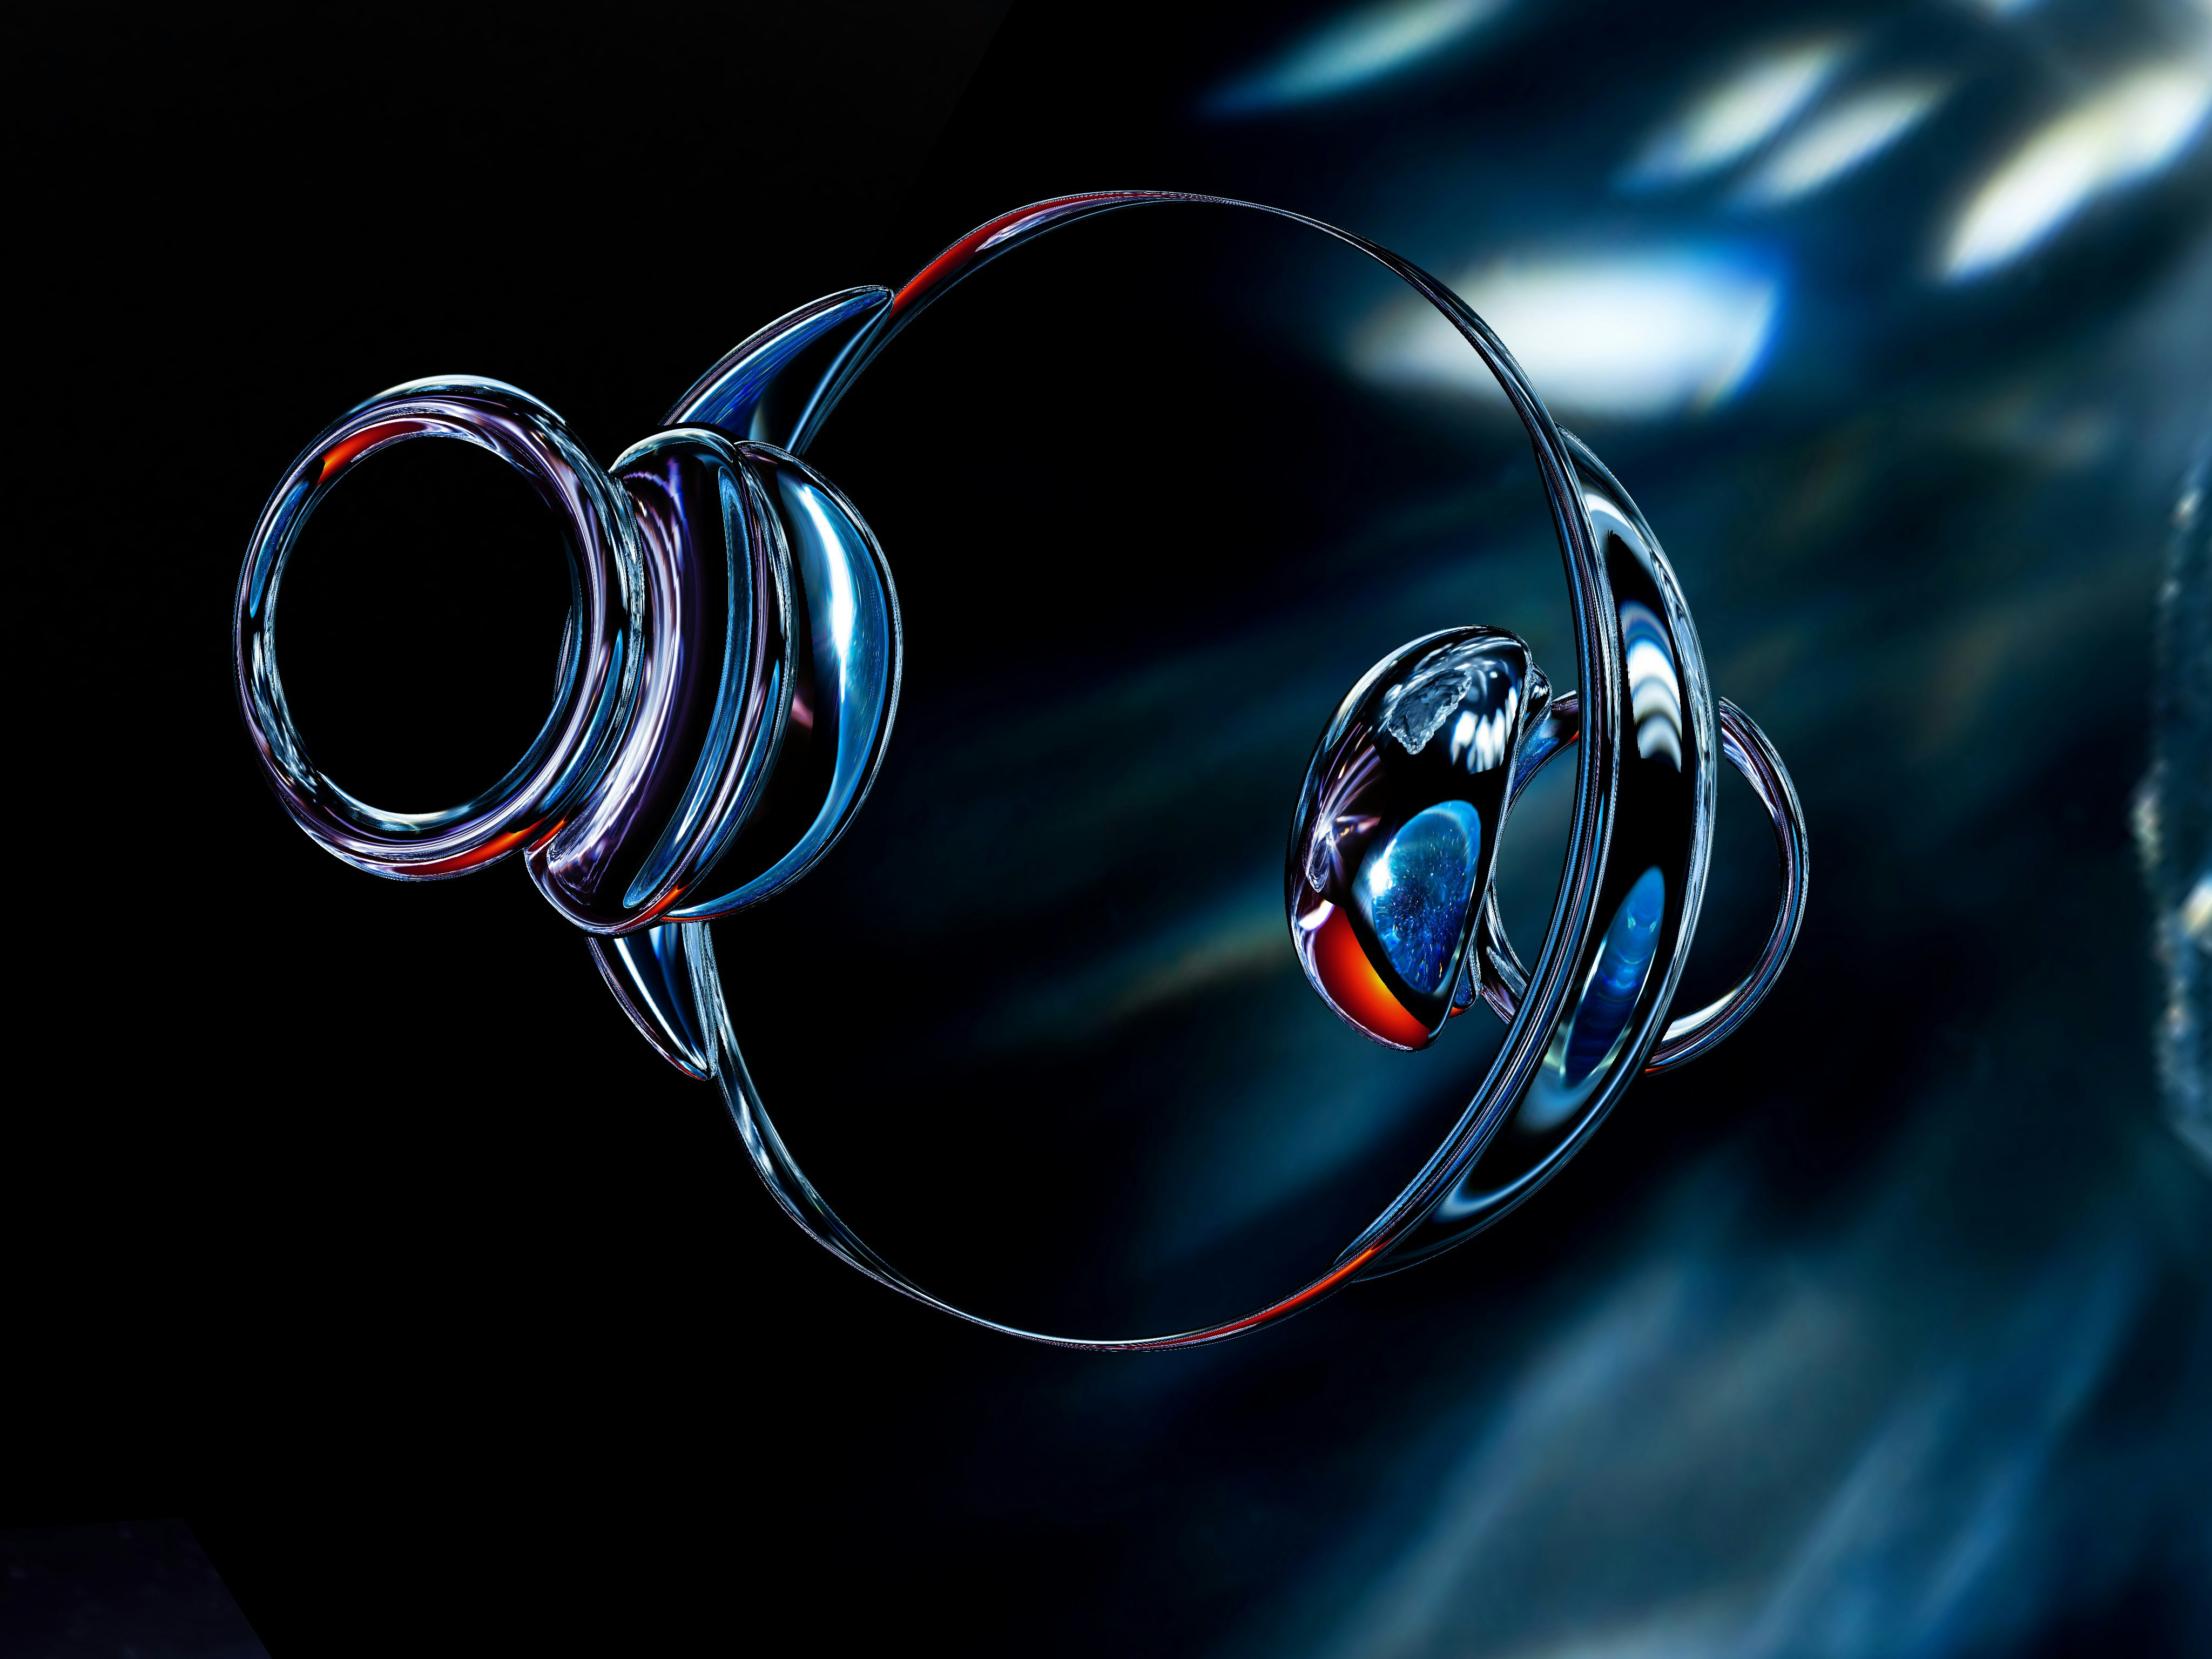
\includegraphics[width=1\paperwidth,height=0.5\paperheight]{img/luis-vasconcelos-wxj729MaPRY-unsplash.jpg}};%height=0.5\paperheight %% https://unsplash.com/de/fotos/blaues-und-rotes-licht-digitales-hintergrundbild-wxj729MaPRY
 %\node[opacity=1,inner sep=0pt] at (0.37\paperwidth,0.4\paperheight){
\includegraphics[scale=0.5]{img/gau-1.pdf}};
 \node at (0.25\paperwidth, 0.45\paperheight) {
\includegraphics[scale=0.65]{img/gau-1.pdf}};
\end{tikzpicture}}
}

\makeatletter                   
\def\printauthor{%                  
    {\large \@author}}          
\makeatother

\begin{titlepage}
\BgThispage
\newgeometry{left=00.5cm,right=6cm,bottom=3cm}
\vspace*{0.25\textheight}
\noindent
\hspace{0.5cm}
\textcolor{white}{\Huge\textbf{\textsf{\maniflow}}} %the titles
\vspace*{0.25cm}\par
\hspace{-0.055cm}
\textcolor{white}{\large\textbf{\textsf{A Python library for geometric processing}}}
\hspace{-20pt}
\vspace*{10cm}\par
\noindent
\hspace*{0.4\paperwidth}
\begin{minipage}{0.4\linewidth} %author info
    \begin{flushright}
        \printauthor
    \end{flushright}
\end{minipage} \hspace{15pt}
%
\begin{minipage}{0.9\linewidth} %the ornament
    \hspace{-0.5cm}
    \begin{tikzpicture}
        \node[rotate=90] at (0,0) {\pgfornament[width=3cm, color=titlepagecolor]{86}};
    \end{tikzpicture}
\end{minipage} \hspace{-10pt}
%
\end{titlepage}
\pagenumbering{arabic}
\pagenumbering{gobble}
\begin{abstract}
    The purpose of this library is to provide tools for the study of the most beautiful discipline of mathematics: geometry and geometric analysis. In doing so, we restrict ourselves to 2-manifolds. For a mathematician, this may initially seem like a major restriction. However, it allows us, in a relatively simple way, to represent 2-manifolds as ''meshes`` and to develop powerful tools to study them. 
    
    The abstraction hardly needs to be restricted at all, because the proposed calculus for meshes makes it possible to develop new geometries with comparatively little effort. Properties of these meshes can then be examined using \maniflow. For example, we provide tools to break down meshes into their connected components. You can also use \maniflow{} to determine the orientability of a mesh. It is also possible to run a geometric flow, such as the mean curvature flow, on a mesh. This means that \maniflow{} can also be used to examine meshes with regard to curvature (Gaussian curvature, mean curvature).
    
    \maniflow{} also provides the option of creating images of the meshes. This makes it possible, for example, to create animations of geometric flows etc.
\end{abstract}
\tableofcontents
\listoffigures
\vfill
\hrule\vspace*{0.2cm}
\noindent\footnotesize{\maniflow{} was developed as part of the course M.Mat.0731 ''Advanced practical course in scientific computing`` at Georg-August University Göttingen.

The image on the frontpage is taken from \href{https://unsplash.com/de/fotos/blaues-und-rotes-licht-digitales-hintergrundbild-wxj729MaPRY}{\url{https://unsplash.com/de/fotos/blaues-und-rotes-licht-digitales-hintergrundbild-wxj729MaPRY}}
\restoregeometry
\normalsize
\pagenumbering{arabic}
\newpage
\section*{Getting started}
\addcontentsline{toc}{section}{Getting started}
\epigraph{\footnotesize{``Be patient, for the world is broad and wide.``}}{\footnotesize{-- \textsc{E. A. Abbott}, Flatland: A Romance of Many Dimensions }}
The code of \maniflow{} was originally published on
\begin{center}
    \qrcode{https://gitlab.gwdg.de/yangshan.xiang/scientific-computing}\\
    \vspace*{0.5cm}
    \href{https://gitlab.gwdg.de/yangshan.xiang/scientific-computing}{\url{https://gitlab.gwdg.de/yangshan.xiang/scientific-computing}}
\end{center}
To install the libary, simply use
\begin{center}
    \boxedcode{\texttt{pip install dist/maniflow-1.0-py2.py3-none-any.whl}}
\end{center}
To build the wheel file of the library, use
\begin{center}
    \boxedcode{\texttt{python setup.py bdist\_wheel --universal}}
\end{center}
\paragraph{Dependencies.} The installation and usage of \maniflow{} requires the following packages to be installed: \href{https://numpy.org/}{\texttt{numpy}}, \href{https://pillow.readthedocs.io/en/stable/}{\texttt{pillow}}
\paragraph{Optional dependencies.} When using \texttt{maniflow.render.SVGPainterRenderer}, one requires the installation of \href{https://pypi.org/project/drawsvg/}{\texttt{drawsvg}}.
\section{Introduction}
First, we will look at the basic mathematical concepts that ultimately underpin the whole theory. So let's start with so-called meshes and look at some examples and how these mathematical concepts can be implemented in code using \maniflow{}.
\begin{defi}[Mesh]
    Let $V$ be a vector space  over $\R$ of dimension $n$. Let $\mathcal{V}_M\subset V$ be a set of points in $V$. We further let $\mathcal{F}_M\subset\mathcal{V}_M^3$. The pair $M = (\mathcal{V}_M, \mathcal{F}_M)$ is then called mesh. The elements of $\mathcal{V}_M$ are called points of $M$ and the elements of $\mathcal{F}_M$ are the faces of the mesh $M$.
\end{defi}
For a mesh $M = (\mathcal{V}_M, \mathcal{F}_M)$ we will often denote $V_M = \vert\mathcal{V}_M\vert$ and $F_M = \vert\mathcal{F}_M\vert$.
\paragraph{Remark.} Meshes $M$ can be considered as $2$-dimensional simplicial complexes. Thus for $2$-dimensional manifolds $\Tilde{M}\subset V$ we may find a \textit{triangulation} simplicial complex $K$ of $\Tilde{M}$. The corresponding mesh will be called \textit{triangulation} mesh of the manifold $\Tilde{M}$.
\begin{ex}[Tetrahedron]\label{ex:tetra} Let 
\begin{align*}
    \mathcal{V} = \left\{\left(\sqrt{\frac89},0,-\frac13\right),\left(-\sqrt{\frac29},\sqrt{\frac23},-\frac13\right),\left(-\sqrt{\frac29},-\sqrt{\frac23},-\frac13\right), \left(0,0,1\right)\right\}\subset\R^3
\end{align*}
and $\mathcal{F} = \{f\in2^{\mathcal{V}}:\vert f\vert = 3\}$. The mesh $T = (\mathcal{V},\mathcal{F})$ is the tetrahedron, which is displayed in figure \ref{fig:tetra}.
    \begin{figure}[h]
        \centering
        \includesvg[scale=0.6]{img/tetrahedron.svg}
        \caption{Tetrahedron}
        \label{fig:tetra}
    \end{figure}
This can be implemented using \texttt{maniflow} by using the \texttt{Mesh} class:
\begin{lstlisting}
import numpy as np
import itertools
from maniflow.mesh import Mesh, Face

# computing the four vertices of the tetrahedron
v1 = np.array([np.sqrt(8/9), 0, -1/3])
v2 = np.array([-np.sqrt(2/9), np.sqrt(2/3), -1/3])
v3 = np.array([-np.sqrt(2/9), -np.sqrt(2/3), -1/3])
v4 = np.array([0, 0, 1])

tetra = Mesh()
# setting the vertices as the vertices of the new mesh object
tetra.vertices = [v1, v2, v3, v4]
# now we compute the subsets of all the vertices consiting of three vertices
subsets = set(itertools.combinations(list(range(tetra.v)), 3))
# the faces are then set as the faces of tetra
tetra.faces = [Face(tetra, *list(i)) for i in subsets]
\end{lstlisting}
This way, we obtain the \texttt{Mesh} object \texttt{tetra} which represents a tetrahedron.
\end{ex}
\subsection{Reading and writing \texttt{.obj} files}\label{sec:objfiles}
The repeated computation of meshes can require a lot of computing capacity under certain circumstances. It can also be difficult to programme complicated geometries line by line in the code. To avoid these difficulties, \maniflow{} supports the \texttt{.obj} file format.
This makes it possible to export meshes for further editing in other programmes (e.g. \href{https://www.blender.org/}{Blender} or similar) or to display them\footnote{if you do not want to use the internal renderer of \maniflow{}}.
You can also use third-party software to create complicated geometries relatively easily and import them into \maniflow{}.
Interaction with .obj files is made possible by the maniflow.mesh.obj.OBJFile class.
\paragraph{Caution:} \texttt{maniflow.mesh.obj.OBJFile} currently disregards any normal vectors, texture coordinates, line elements etc. defined in the \texttt{.obj} file.
Only the coordinates of the vertices are taken into account and for the faces only the indices of the vertices that make them up are taken into consideration.
\begin{ex}
    Consider the \texttt{Mesh} object \texttt{tetra} from example \ref{ex:tetra}. To store this mesh in a \texttt{.obj} file, we may use
    \begin{lstlisting}
from maniflow.mesh.obj import OBJFile

OBJFile.write(tetra, "examples/tetrahedron.obj")
    \end{lstlisting}
    This code produces the file \url{examples/tetrahedron.obj}. In order to load a mesh into \maniflow{}, simply use
    \begin{lstlisting}
mesh = OBJFile.read("examples/tetrahedron.obj")
    \end{lstlisting}
\end{ex}
\subsection{\texttt{maniflow.mesh.utils.VertexFunction} -- Creating meshes from parameterisations}
The way we created a mesh of a tetrahedron in the previous example is very static and absolutely not suitable if you want to study more complicated geometries. \maniflow{}, however, provides the option of creating meshes quite easily using parameterisations. For this purpose, \maniflow{} provides the wrapper \texttt{maniflow.mesh.utils.VertexFunction}, which executes a given function on all vertices of the mesh and has the resulting mesh as output.
\begin{ex}
    For the following example, we assume that we have a \texttt{Mesh}-object \code{mesh} and we want to shift this mesh by the vector $\begin{pmatrix}1 & 2 & 3\end{pmatrix}^{\intercal}\in\R^3$. For this we make use of a \texttt{VertexFunction}:
    \begin{lstlisting}
# importing the wrapper from maniflow.mesh.utils
from maniflow.mesh.utils import VertexFunction

# implementing the VertexFuntion 'shift'
@VertexFuntion
def shift(vertex):
    return vertex + np.array([1, 2, 3])


# applying 'shift' to 'mesh'
shifted = shift(mesh)
    \end{lstlisting}
    The resulting \texttt{Mesh}, \code{shifted}, is \code{mesh} shifted by the vector $\begin{pmatrix}1 & 2 & 3\end{pmatrix}^{\intercal}\in\R^3$.
\end{ex}
Another application of this would be the creation of meshes from parameterisations $\psi\colon \R^2\supset D\to\R^3$. Oftentimes, the domain $D$ is a cartesian product of two intervals, so $D = I_1\times I_2$.\footnote{Or to be more precise, \maniflow{} makes it easy to create meshes from parametrisations, where the domain $D$ is homoeomorphic to a square.} For this, \maniflow{} provides the class \texttt{maniflow.mesh.parameterized.Grid}.
\begin{ex}[Moebius strip]\label{ex:moebius_creation}
We now turn to an example where we want to create a triangulation of a moebius strip. To this end, we will use the parametrisation
\begin{align*}
    \psi\colon [0, 2\pi]\times [-1,1]\to\R^3,\ (u,v)\mapsto\begin{pmatrix}
        \left(1+\frac{v}{2}\cos{\frac{u}{2}}\right)\cos{u}\\
        \left(1+\frac{v}{2}\cos{\frac{u}{2}}\right)\sin{u}\\
        \frac{v}{2}\sin{\frac{u}{2}}
    \end{pmatrix}.
\end{align*}
In order to discretise the set $[0,2\pi]\times[-1,1]$, we make use of \texttt{maniflow.mesh.parametrized.Grid} in order to create a high resolution lattice. Then we can implement a \texttt{VertexFunction} to capture the parametrisation $\psi$ in code and apply it to our lattice.
\begin{lstlisting}
from maniflow.mesh.parameterized import Grid
from maniflow.mesh.utils import VertexFunction


# implementing the parametrisation 1:1 in code as a VertexFunction
@VertexFunction
def moebius(vertex):
    x = vertex[0]
    y = vertex[1]
    x0 = np.cos(x) * (1 + (y / 2) * np.cos(x / 2))
    x1 = np.sin(x) * (1 + (y / 2) * np.cos(x / 2))
    x2 = (y / 2) * np.sin(x / 2)
    return np.array([x0, x1, x2])


u = Grid((0, 2 * np.pi), (-1, 1), 30, 10)  # create a high resolution grid
moebiusMesh = moebius(u)  # mapping the vertices from the grid according to the parametrisation
coincidingVertices(moebiusMesh) # remove the redundant vertices at the joint after making the moebius band
\end{lstlisting}
With this we obtain the \texttt{Mesh}-object \code{moebiusMesh}. Using \texttt{maniflow.mesh.obj.OBJFile}, we can write this mesh to memory as a \texttt{.obj} file, see section \ref{sec:objfiles}
\begin{lstlisting}
from maniflow.mesh.obj import OBJFile

OBJFile.write(moebiusMesh, "examples/moebius.obj")
\end{lstlisting}
Unsurprisingly, one can then load this file into \href{https://www.blender.org/}{Blender} and create pictures of it etc.\footnote{\maniflow{} comes with its own simple renderer. But if you want to do more elaborated computer graphics, you might consider using some other software to render images.} Figure \ref{fig:moubius_blender} shows a screenshot taken from Blender with the \texttt{.obj} file from \href{https://gitlab.gwdg.de/yangshan.xiang/scientific-computing/-/blob/82c42c864b3e46303b208b78720b8109116c78da/examples/moebius.obj}{\url{examples/moebius.obj}}.
\end{ex}
\begin{figure}[t]
    \centering
    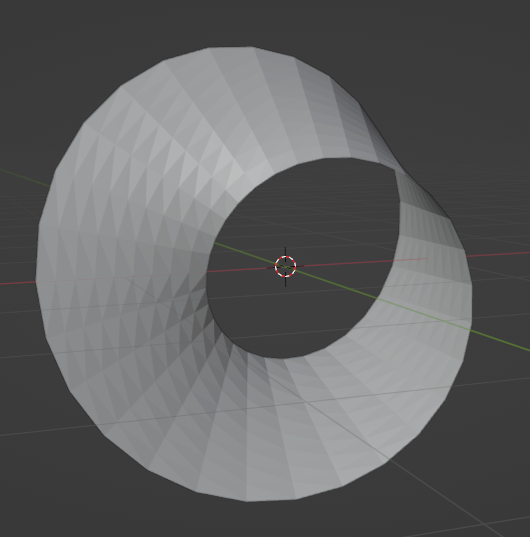
\includegraphics[scale=0.35]{img/moebius_2023-05-23.png}
    \caption{Screenshot of \href{https://www.blender.org/}{Blender} with a moebius strip made with \maniflow{}}
    \label{fig:moubius_blender}
\end{figure}
\newpage
\section{The face graph of a mesh}
\begin{defi}[Undirected Graph]
    Let $\V_G$ be a set and $\E_G\subset\{e\in2^{\V_G}: |e|=2\}$ be a set of unordered pairs of elements from $\V_G$. The pair $G = (\V_G, \E_G)$ is then called undirected Graph. The elements from $\V_G$ are called vertices of $G$ and the elements from $\E_G$ are called edges of $G$.
\end{defi}
For a Graph $G=(\V_G,\E_G)$ we write
\begin{align*}
    \vcenter{\hbox{\begin{tikzpicture}
    \node (A) at (0,0) {$x$};
    \node (B) at (1,0) {$y$};
    \draw[-] (A) -- (B);\end{tikzpicture}}}
\end{align*}
if $\{x,y\}\in\E_G$. If we take all edges and points together in this way, we get the picture
of a graph with undirected edges.
\begin{ex}
    \begin{equation}\label{eq:sample_g}
    G\colon\left(\vcenter{\hbox{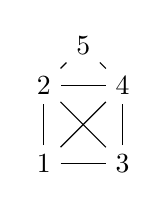
\begin{tikzpicture}[scale=0.5]
    \node (1) at (-1,-1) {$1$};
    \node (2) at (-1,1) {$2$};
    \node (3) at (1,-1) {$3$};
    \node (4) at (1,1) {$4$};
    \node (5) at (0,2) {$5$};
    \draw[-] (1) -- (2);
    \draw[-] (2) -- (3);
    \draw[-] (3) -- (4);
    \draw[-] (4) -- (2);
    \draw[-] (2) -- (5);
    \draw[-] (5) -- (4);
    \draw[-] (4) -- (1);
    \draw[-] (1) -- (3);
\end{tikzpicture}}}\right),\qquad H\colon\left(\vcenter{\hbox{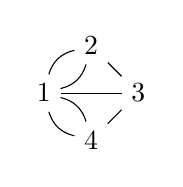
\begin{tikzpicture}[scale=0.6]
\node (1) at (-1, 0) {$1$};
\node (2) at (0, 1) {$2$};
\node (3) at (1,0) {$3$};
\node (4) at (0,-1) {$4$};
\draw[-] (1) -- (3);
\path [-] (1) edge[bend right=-30](2); 
\path [-] (1) edge[bend right=30](2); 
\path [-] (1) edge[bend right=-30](4); 
\path [-] (1) edge[bend right=30](4);
\draw[-] (3) -- (2);
\draw[-] (4) -- (3);
\end{tikzpicture}}}\right)
\end{equation}
\end{ex}
\begin{defi}[Face Graph]
    Let $M = (\mathcal{V}_M, \mathcal{F}_M)$ be a mesh and
    \begin{align*}
        \mathcal{E} = \left\{(f_1,f_2)\in\mathcal{F}_G^2: \vert f_1\cap f_2\vert =2\right\}
    \end{align*}
    The face graph of $M$ is the graph $(\mathcal{F}_M,\mathcal{E})$.
\end{defi}
\begin{ex} The face graph of the tetrahedron is given by
    \begin{equation}\label{eq:sample_g1}
    G\colon\left(\vcenter{\hbox{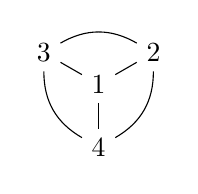
\begin{tikzpicture}[scale=0.8]
    \node (1) at (0,0) {$1$};
    \node (2) at (0.87,0.5) {$2$};
    \node (3) at (-0.87,0.5) {$3$};
    \node (4) at (0,-1) {$4$};
    \draw[-] (1) -- (2);
    \draw[-] (1) -- (3);
    \draw[-] (1) -- (4);
    \path[-] (2) edge[bend right=30] (3);
    \path[-] (3) edge[bend right=30] (4);
    \path[-] (4) edge[bend right=30] (2);
\end{tikzpicture}}}\right)
\end{equation}
\end{ex}
The face graph of a given mesh can be constructed by algorithm \ref{alg:facegraph}.
\begin{algorithm}
    \SetKwInOut{Input}{Input}
    \SetKwInOut{Output}{Output}

    \Input{A mesh $M = (\mathcal{V}_M, \mathcal{F}_M=\{f_1,f_2,f_3\ldots\})$}
    \Output{The adjacency matrix of the face graph of the mesh $M$}
    \caption{Construction of the face graph of a given mesh}
    \label{alg:facegraph}
    $G := 0\in\R^{F_M\times F_M}$\;
    \For{$i=1$ \KwTo $F_M$}
    {
        $neighbors := 0$\;
        \For{$j=1$ \KwTo $F_M$}
        {
            \If{$neighbors = 3$}{
            \textbf{break}\;
            }
            \If{$\vert f_i\cap f_j\vert = 2$ \normalfont{\textbf{and}} $i\neq j$}{
            $G_{ij} \leftarrow 1$\;
            $neighbors \leftarrow neighbors + 1$\;
            }
        }
    }
    \Return{$G$}
\end{algorithm}
Since this algorithm loops over the faces of the mesh in a nested way, the complexity of it lies in $O(F_M^2)$. As this runtime complexity has the consequence of the algorithm being very slow at execution for somewhat large meshes, the face graph is computed dynamically by \texttt{maniflow.mesh.Mesh.faceGraph}.
\subsection{A first application: \texttt{maniflow.mesh.utils.connectedComponents}}
The method \texttt{maniflow.mesh.utils.connectedComponents} decomposes the given mesh into its connected components. Now that we have an algorithm with which to compute the face graph, the connected components of a mesh can now be identified as the connected components of the face graph. These can be determined via the breadth-first traversal of the face graph. 
\begin{algorithm}
    \SetKwInOut{Input}{Input}
    \SetKwInOut{Output}{Output}

    \Input{A mesh $M = (\mathcal{V}_M, \mathcal{F}_M=\{f_1,f_2,f_3\ldots\})$}
    \Output{The connected components of the mesh $M$}
    \caption{Construction of the face graph of a given mesh}
    \label{alg:components}
    Compute the adjacency matrix $G$ using \ref{alg:facegraph}\;
    $start := 1$\;
    $n := 1$\;
    \While{$\mathcal{F}_M\neq\emptyset$}{
        Compute a breadth first traversal sequence $T_n \leftarrow \{f_{start}, f_b,f_c,\ldots\}\subseteq\mathcal{F}_M$\;
        $n \leftarrow n+1$\;
        $\mathcal{F}_M\leftarrow \mathcal{F}_M\setminus T_n$\;
        Set $1< start\leq F_M$ such that $f_{start}\in\mathcal{F}_M$\;
    }
    
    \Return{$T_1$, $T_2$, $\ldots$}
\end{algorithm}
\paragraph{Runtime analysis.} Algorithm \ref{alg:facegraph} has a runtime complexity which lies in $O(F_M^2)$. The breadth-first traversal on the face graph has a runtime\footnote{Since on a graph with the number of vertices being $V$ and the number of edges being $E$ the breadth first search has a complexity of $O(E + V)$. As every face has at most three neighbors we obtain the given runtime complexity.} complexity of $O(F_M + 3\cdot F_M) = O(F_M)$. The computation of $\mathcal{F}_M\setminus T_n$ has also quadratic complexity $O(\vert\mathcal{F}_M\vert^2)$. Thus the overall complexity of algorithm \ref{alg:components} lies in $O(F_G^2)$.
\begin{ex}
    In this example we analyse the connected components of the teapot from \texttt{examples/teapot.obj}. The teapot is displayed in figure \ref{fig:teapot}.
    \begin{figure}[h]
        \centering
        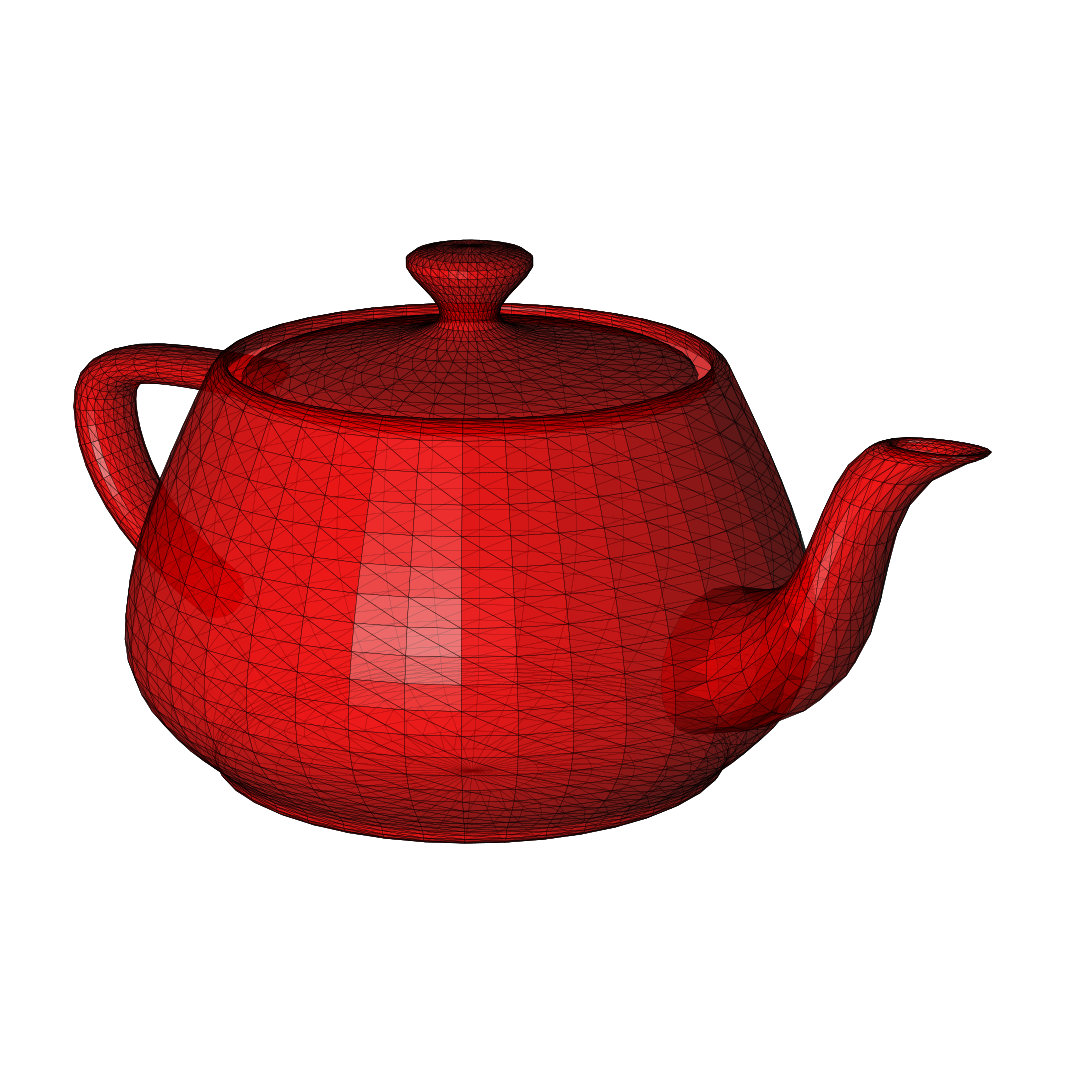
\includegraphics[scale=0.15]{img/teapot.png}
        \caption{The teapot from \texttt{examples/teapot.obj}}
        \label{fig:teapot}
    \end{figure}
    \newline\noindent The connected components can be computed using the following code
    \begin{lstlisting}
from maniflow.mesh import Mesh
from maniflow.mesh.obj import OBJFile
from maniflow.mesh.utils import connectedComponents, coincidingVertices

teapot = OBJFile.read("examples/teapot.obj")  # reading the mesh from memory
coincidingVertices(teapot)  # identifying and collapsing coinciding vertices

# now we compute the connected components
components = connectedComponents(teapot)

# we can now reconstruct meshes from these lists of faces and write them to .obj files
for i, component_list in enumerate(components):
    component = Mesh.fromFaceList(teapot, *component_list)
    OBJFile.write(component, "teapot" + str(i + 1) + ".obj")
    \end{lstlisting}
    The resulting components are shown in figure \ref{fig:teapotcomps}.
    \begin{figure}[ht]
    \centering
    \subfloat[The lid of the teapot]{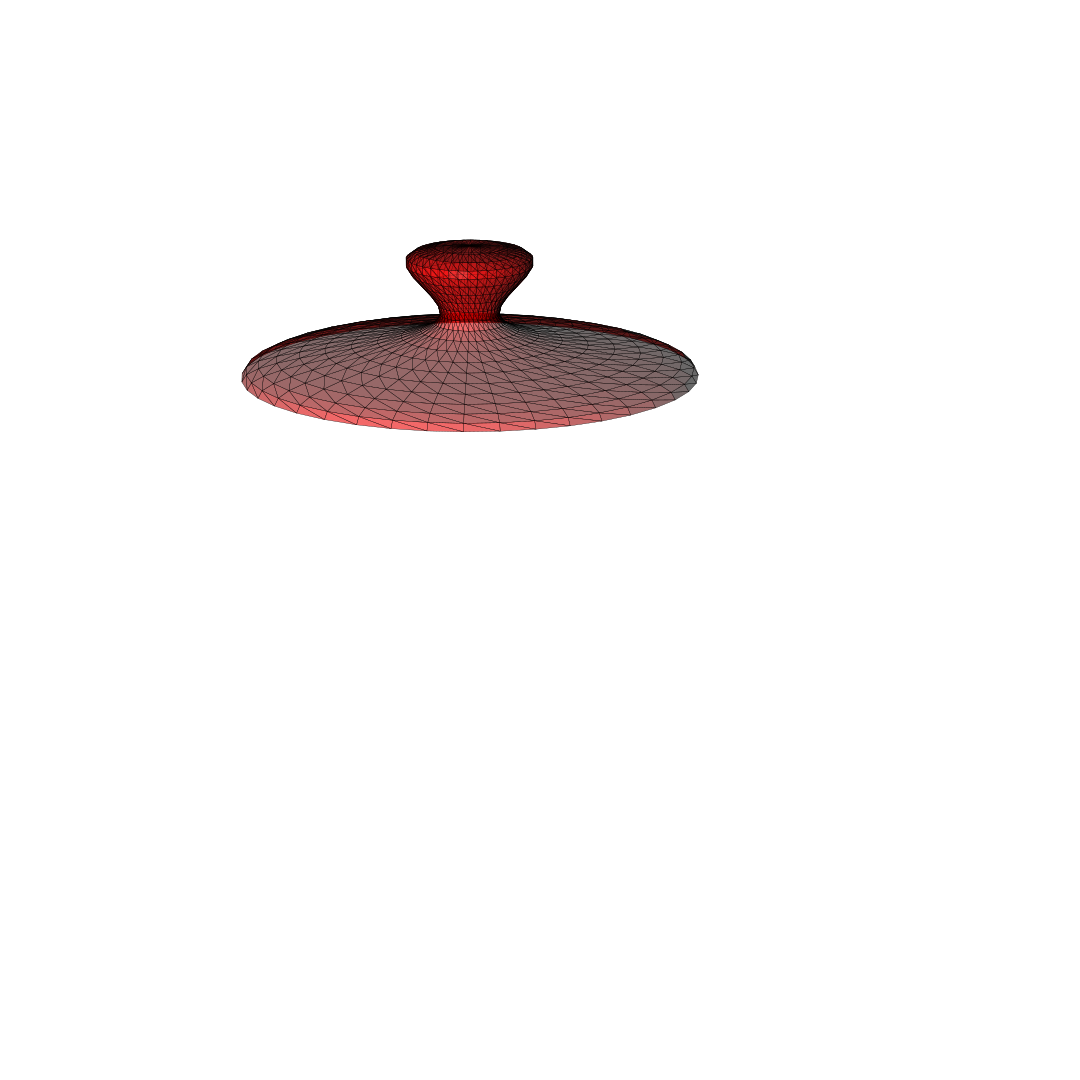
\includegraphics[width=0.4\textwidth]{img/teapot1.png}}\hfil
    \subfloat[The handle of the teapot]{
\includegraphics[width=0.4\textwidth]{img/teapot2.png}}\hfil\\
    \subfloat[The body of the teapot]{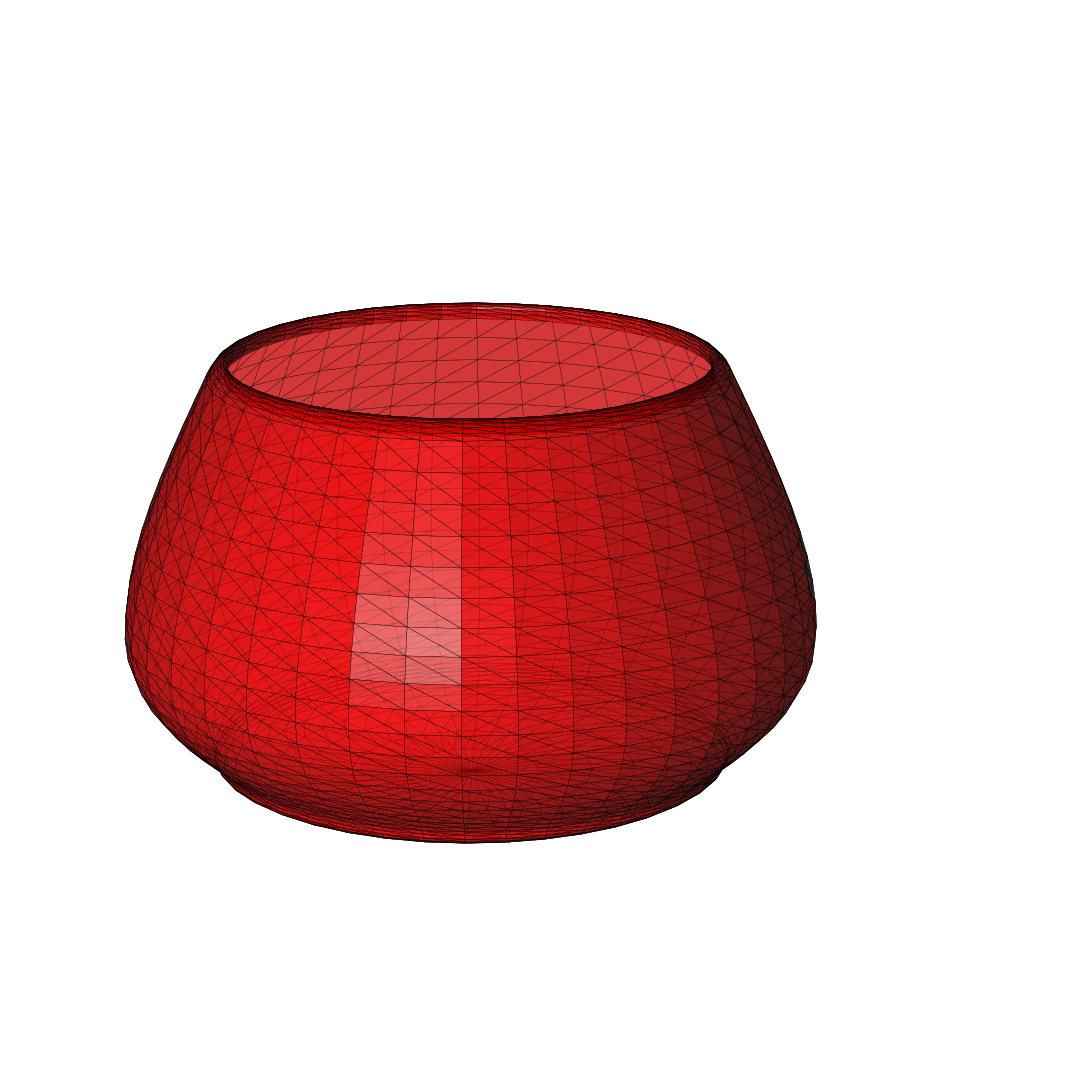
\includegraphics[width=0.4\textwidth]{img/teapot3.png}}\hfil
    \subfloat[The spout of the teapot]{
\includegraphics[width=0.4\textwidth]{img/teapot4.png}}\hfil
    \caption{The connected components of the teapot}
    \label{fig:teapotcomps}
\end{figure}
\end{ex}
\subsection{Another application: checking orientability of a \texttt{Mesh}}
Orientability is an important property of manifolds in geometry. For example, the area can only be meaningfully defined for orientable 2-manifolds. For 2-manifolds embedded in $\R^3$, orientability is equivalent to the existence of a continuous unit-normal vector field on the manifold. Similarly, we can extend the notion of orientability to meshes. If we consider a face spanned by the vertices $v_1,\ v_2$ and $v_3$, the normal vector is, for example given by\footnote{Note that $n$ does not necessarily have length $1$. But one may always obtain a unit normal vector by rescaling}
\begin{align*}
    n = (v_1 - v_2)\times (v_1 - v_3).
\end{align*}
Hence, the orientation or direction of $n$ is dependent upon the enumeration of the vertices that define the face. A priori it is not clear that two neighboring faces really do have ``compatible'' enumerations of their vertices. So it may happen that two neighboring faces have normal vectors that point in ``opposite'' directions.\footnote{An appeal to the reader's intuition. You have to be careful with these notions.}
\begin{defi}[Orientation of faces]
    Let $f = (v_1, v_2, v_3)$ be a face defined by the vertices $v_i$ for $1\leq i\leq 3$. Let $f'$ be another face that is defined by the vertices $v_1,\ v_2$ and $v_{\ast}$. We say that two faces have the same orientation, if there is a cyclic permutation $\sigma\in S_3$ such that
    \begin{align*}
        (f_1, f_2) = (f'_{\sigma(2)},f'_{\sigma(1)}).
    \end{align*}
    Where $f_i$ and $f'_i$ denote the $i$-th vertex in the faces $f$ and $f'$ respectively.
\end{defi}
In other words, two faces have the same orientation if they share an edge and that edge is traversed in opposite directions, when listing the vertices of the faces, see figure \ref{fig:orientation}.
\begin{ex}
    Consider the faces $f = (1, 2, 3)$ and $f' = (2, 3, 4)$. Then $f$ and $f'$ share the edge made up of the vertices $2$ and $3$. But both of them traverse this edge in the same direction $(2,3)$. On the other hand, if we changed the enumeration of $f'$ to $(3, 2, 4)$, the faces would have matching orientation. This is exactly the situation depicted in figure \ref{fig:orientation}.
\end{ex}
\begin{figure}[ht]
    \centering
    \subfloat[Non compatible orientation]{
    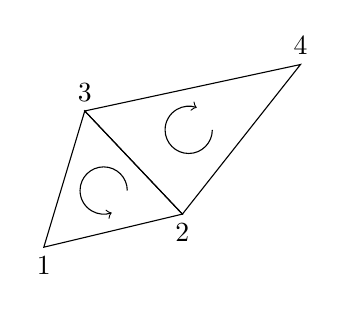
\begin{tikzpicture}
        \draw[]{} (-1.1, -1.13) -- (0.66, -0.71) node[below]{$2$} -- (-0.58, 0.6) node[above]{$3$} -- cycle node[below]{$1$};
        \draw[]{} (0.66, -0.71) -- (-0.58, 0.6) -- (2.16, 1.19) node[above]{$4$} -- cycle;
        \draw[->] (-0.04,-0.41) arc[radius=0.3cm,start angle=0,delta angle=290];
        \draw[->] (1.04,0.36) arc[radius=0.3cm,start angle=0,delta angle=-290];
    \end{tikzpicture}
    }
    \subfloat[Compatible orientation]{
    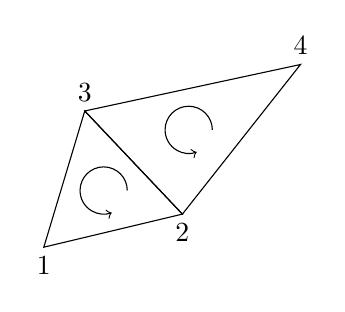
\begin{tikzpicture}
        \draw[]{} (-1.1, -1.13) -- (0.66, -0.71) node[below]{$2$} -- (-0.58, 0.6) node[above]{$3$} -- cycle node[below]{$1$};
        \draw[]{} (0.66, -0.71) -- (-0.58, 0.6) -- (2.16, 1.19) node[above]{$4$} -- cycle;
        \draw[->] (-0.04,-0.41) arc[radius=0.3cm,start angle=0,delta angle=290];
        \draw[->] (1.04,0.36) arc[radius=0.3cm,start angle=0,delta angle=290];
    \end{tikzpicture}
    }
    \caption{Two triangles with compatible and non compatible orientations}
    \label{fig:orientation}
\end{figure}
In order to determine whether a given mesh is orientable or not, we can sort of ``push'' an orientation to the mesh by traversing each of the faces in breadth-first traversal and adjusting the orientations / enumerations of vertices of each of the neighboring faces for the currently traversed face.\footnote{Of course we have to remember the faces we already considered while traversing the mesh in order to avoid faces being re-oriented twice.}
\begin{algorithm}
    \SetKwInOut{Input}{Input}
    \SetKwInOut{Output}{Output}

    \Input{A mesh $M = (\mathcal{V}_M, \mathcal{F}_M=\{f_1,f_2,f_3\ldots\})$}
    \caption{Pushing an orientation to a mesh}
    \label{alg:pushorientation}
    Store the connected components of $M$ in $\mathcal{C}$ (see algorithm \ref{alg:components})\;
    \For{$c\in\mathcal{C}$}{
    $visited := \emptyset$\;
    \For{$f\in c$}{
    \If{$f\notin visited$}{
    Store neighbouring faces to $f$ in $neighbours$\;
    \For{$f_n\in neighbours$}{
    \If{$f$ and $f_n$ do not have compatible orientations}{
    reverse the enumeration of vertices in $f_n$\;
    }
    }
    $visited \leftarrow visited \cup \{ f\}$\;
    }
    }
    }
\end{algorithm}
This is what algorithm \ref{alg:pushorientation} does. The method \texttt{maniflow.mesh.utils.pushOrientation} implements this algorithm in \maniflow{}.
Finally, to check whether a mesh is orientable or not, we only need to iterate over all surfaces in the mesh and ask whether all neighbours have a compatible orientation. This is implemented as the method \texttt{maniflow.mesh.utils.isOrientable}.
\paragraph{Runtime analysis.}  Algorithm \ref{alg:pushorientation} has a complexity of $O(F_M^2)$. % TODO: more details?
\begin{ex}[Orientability of the Moebius strip]
    Consider the \texttt{Mesh} object \texttt{moebiusMesh} from example \ref{ex:moebius_creation}. To determine whether this mesh is orientable or not, use
    \begin{lstlisting}
from maniflow.mesh.utils import isOrientable

print(isOrientable(moebiusMesh))
    \end{lstlisting}
    As expected, the output will be \texttt{False} as the Moebius strip is not orientable.
\end{ex}
\noindent Another example that is less trivial than the Moebius strip is documented in the file \href{https://gitlab.gwdg.de/yangshan.xiang/scientific-computing/-/blob/28846b92bf3f99fa84b650267886782c43791715/examples/roman_surface.ipynb}{\url{examples/roman\_surface.ipynb}} where the so-called Roman surface is discussed.

\documentclass{article}
\usepackage[utf8]{inputenc}
\usepackage{amsmath}
\usepackage{amsfonts}
\usepackage{graphicx}
\usepackage{amssymb}
\usepackage{amsthm}
\usepackage{float}
\usepackage{tikz}
\usepackage{mlmodern}
\usepackage{subfig}
\usepackage[T1]{fontenc}
\usepackage[left=2.5cm,right=2.5cm]{geometry}
\usepackage[linesnumbered,ruled]{algorithm2e}

\usepackage{svg}

\usepackage{listings}
\newcommand{\code}[1]{\texttt{#1}} % inline code setting
\renewcommand{\lstlistingname}{Code}

\definecolor{codebg}{RGB}{230,230,230}
\lstset {
    breakatwhitespace=false,         % sets if automatic breaks should only happen at whitespace
    breaklines=true,                 % sets automatic line breaking
    captionpos=b,                    % sets the caption-position to bottom
    tabsize=4,
    %showstringspaces=false,
    numbers=left,                    % where to put the line-numbers; possible values are (none, left, right)
    numbersep=2pt,                   % how far the line-numbers are from the code
    numberstyle=\tiny, % the style that is used for the line-numbers
    %upquote=true,
    backgroundcolor = \color{codebg},
    basicstyle=\small\ttfamily, % basic font setting
    emph={int,char,double,float,unsigned,void,bool},
    %emphstyle={\color{blue}},
    escapechar=\&,
    columns=fixed
}

\newtheorem{defi}{Definition}
\newtheorem{ex}{Example}
\newtheorem{prop}{Proposition}
\newtheorem{theorem}{Theorem}
\newtheorem{lemma}{Lemma}
\newtheorem{kor}{Corollary}

\newcommand{\N}{\mathbb{N}}

\newcommand{\R}{\mathbb{R}}
\newcommand{\V}{\mathcal{V}}
\newcommand{\E}{\mathcal{E}}

\title{\texttt{maniflow} -- a (partial) documentation}
\author{Felix Widmaier}
\date{}


\begin{document}
\maketitle
\section{Introduction}
\begin{defi}[Mesh]
    Let $V$ be a vector space  over $\R$ of dimension $n$. Let $\mathcal{V}_M\subset V$ be a set of points in $V$. We further let $\mathcal{F}_M\subset\mathcal{V}_M^3$. The pair $M = (\mathcal{V}_M, \mathcal{F}_M)$ is then called mesh. The elements of $\mathcal{V}_M$ are called points of $M$ and the elements of $\mathcal{F}_M$ are the faces of the mesh $M$.
\end{defi}
For a mesh $M = (\mathcal{V}_M, \mathcal{F}_M)$ we will often denote $V_M = \vert\mathcal{V}_M\vert$ and $F_M = \vert\mathcal{F}_M\vert$.
\paragraph{Remark.} Meshes $M$ can be considered as $2$-dimensional simplicial complexes. Thus for $2$-dimensional manifolds $\Tilde{M}\subset V$ we may find a \textit{triangulation} simplicial complex $K$ of $\Tilde{M}$. The corresponding mesh will be called \textit{triangulation} mesh of the manifold $\Tilde{M}$.
\begin{ex}[Tetrahedron] Let 
\begin{align*}
    \mathcal{V} = \left\{\left(\sqrt{\frac89},0,-\frac13\right),\left(-\sqrt{\frac29},\sqrt{\frac23},-\frac13\right),\left(-\sqrt{\frac29},-\sqrt{\frac23},-\frac13\right), \left(0,0,1\right)\right\}\subset\R^3
\end{align*}
and $\mathcal{F} = \{f\in2^{\mathcal{V}}:\vert f\vert = 3\}$. The mesh $T = (\mathcal{V},\mathcal{F})$ is the tetrahedron, which is displayed in figure \ref{fig:tetra}.
    \begin{figure}[h]
        \centering
        \includesvg[scale=0.6]{img/tetrahedron.svg}
        \caption{Tetrahedron}
        \label{fig:tetra}
    \end{figure}
This can be implemented using \texttt{maniflow} by using the \texttt{Mesh} class:
\begin{lstlisting}
import numpy as np
import itertools
from maniflow.mesh import Mesh, Face

# computing the four vertices of the tetrahedron
v1 = np.array([np.sqrt(8/9), 0, -1/3])
v2 = np.array([-np.sqrt(2/9), np.sqrt(2/3), -1/3])
v3 = np.array([-np.sqrt(2/9), -np.sqrt(2/3), -1/3])
v4 = np.array([0, 0, 1])

tetra = Mesh()
# setting the vertices as the vertices of the new mesh object
tetra.vertices = [v1, v2, v3, v4]
# now we compute the subsets of all the vertices consiting of three vertices
subsets = set(itertools.combinations(list(range(tetra.v)), 3))
# the faces are then set as the faces of tetra
tetra.faces = [Face(tetra, *list(i)) for i in subsets]
\end{lstlisting}
This way, we obtain the \texttt{Mesh} object \texttt{tetra} which represents a tetrahedron.
\end{ex}
\begin{defi}[Undirected Graph]
    Let $\V_G$ be a set and $\E_G\subset\{e\in2^{\V_G}: |e|=2\}$ be a set of unordered pairs of elements from $\V_G$. The pair $G = (\V_G, \E_G)$ is then called undirected Graph. The elements from $\V_G$ are called vertices of $G$ and the elements from $\E_G$ are called edges of $G$.
\end{defi}
For a Graph $G=(\V_G,\E_G)$ we write
\begin{align*}
    \vcenter{\hbox{\begin{tikzpicture}
    \node (A) at (0,0) {$x$};
    \node (B) at (1,0) {$y$};
    \draw[-] (A) -- (B);\end{tikzpicture}}}
\end{align*}
if $\{x,y\}\in\E_G$. If we take all edges and points together in this way, we get the picture
of a graph with undirected edges.
\begin{ex}
    \begin{equation}\label{eq:sample_g}
    G\colon\left(\vcenter{\hbox{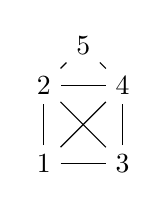
\begin{tikzpicture}[scale=0.5]
    \node (1) at (-1,-1) {$1$};
    \node (2) at (-1,1) {$2$};
    \node (3) at (1,-1) {$3$};
    \node (4) at (1,1) {$4$};
    \node (5) at (0,2) {$5$};
    \draw[-] (1) -- (2);
    \draw[-] (2) -- (3);
    \draw[-] (3) -- (4);
    \draw[-] (4) -- (2);
    \draw[-] (2) -- (5);
    \draw[-] (5) -- (4);
    \draw[-] (4) -- (1);
    \draw[-] (1) -- (3);
\end{tikzpicture}}}\right),\qquad H\colon\left(\vcenter{\hbox{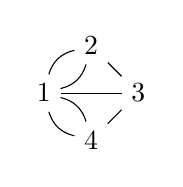
\begin{tikzpicture}[scale=0.6]
\node (1) at (-1, 0) {$1$};
\node (2) at (0, 1) {$2$};
\node (3) at (1,0) {$3$};
\node (4) at (0,-1) {$4$};
\draw[-] (1) -- (3);
\path [-] (1) edge[bend right=-30](2); 
\path [-] (1) edge[bend right=30](2); 
\path [-] (1) edge[bend right=-30](4); 
\path [-] (1) edge[bend right=30](4);
\draw[-] (3) -- (2);
\draw[-] (4) -- (3);
\end{tikzpicture}}}\right)
\end{equation}
\end{ex}
\begin{defi}[Face Graph]
    Let $M = (\mathcal{V}_M, \mathcal{F}_M)$ be a mesh and
    \begin{align*}
        \mathcal{E} = \left\{(f_1,f_2)\in\mathcal{F}_G^2: \vert f_1\cap f_2\vert =2\right\}
    \end{align*}
    The face graph of $M$ is the graph $(\mathcal{F}_M,\mathcal{E})$.
\end{defi}
\begin{ex} The face graph of the tetrahedron is given by
    \begin{equation}\label{eq:sample_g}
    G\colon\left(\vcenter{\hbox{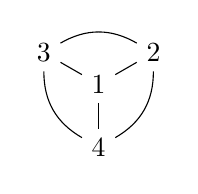
\begin{tikzpicture}[scale=0.8]
    \node (1) at (0,0) {$1$};
    \node (2) at (0.87,0.5) {$2$};
    \node (3) at (-0.87,0.5) {$3$};
    \node (4) at (0,-1) {$4$};
    \draw[-] (1) -- (2);
    \draw[-] (1) -- (3);
    \draw[-] (1) -- (4);
    \path[-] (2) edge[bend right=30] (3);
    \path[-] (3) edge[bend right=30] (4);
    \path[-] (4) edge[bend right=30] (2);
\end{tikzpicture}}}\right)
\end{equation}
\end{ex}
The face graph of a given mesh can be constructed by algorithm \ref{alg:facegraph}.
\begin{algorithm}\label{alg:facegraph}
    \SetKwInOut{Input}{Input}
    \SetKwInOut{Output}{Output}

    \Input{A mesh $M = (\mathcal{V}_M, \mathcal{F}_M=\{f_1,f_2,f_3\ldots\})$}
    \Output{The adjacency matrix of the face graph of the mesh $M$}
    \caption{Construction of the face graph of a given mesh}
    $G := 0\in\R^{F_M\times F_M}$\;
    \For{$i=1$ \KwTo $F_M$}
    {
        $neighbors := 0$\;
        \For{$j=1$ \KwTo $F_M$}
        {
            \If{$neighbors = 3$}{
            \textbf{break}\;
            }
            \If{$\vert f_i\cap f_j\vert = 2$ \normalfont{\textbf{and}} $i\neq j$}{
            $G_{ij} \leftarrow 1$\;
            $neighbors \leftarrow neighbors + 1$\;
            }
        }
    }
    \Return{$G$}
\end{algorithm}
Since this algorithm loops over the faces of the mesh in a nested way, the complexity of it lies in $O(F_M^2)$. As this runtime complexity has the consequence of the algorithm being very slow at execution for somewhat large meshes, the face graph is computed dynamically by \texttt{maniflow.mesh.Mesh.faceGraph}.
\newpage
\subsection{A first application: \texttt{maniflow.mesh.utils.connectedComponents}}
The method \texttt{maniflow.mesh.utils.connectedComponents} decomposes the given mesh into its connected components. Now that we have an algorithm with which to compute the face graph, the connected components of a mesh can now be identified as the connected components of the face graph. These can be determined via the breadth-first traversal of the face graph. 
\begin{algorithm}\label{alg:components}
    \SetKwInOut{Input}{Input}
    \SetKwInOut{Output}{Output}

    \Input{A mesh $M = (\mathcal{V}_M, \mathcal{F}_M=\{f_1,f_2,f_3\ldots\})$}
    \Output{The connected components of the mesh $M$}
    \caption{Construction of the face graph of a given mesh}
    Compute the adjacency matrix $G$ using \ref{alg:facegraph}\;
    $start := 1$\;
    $n := 1$\;
    \While{$\mathcal{F}_M\neq\emptyset$}{
        Compute a breadth first traversal sequence $T_n \leftarrow \{f_{start}, f_b,f_c,\ldots\}\subseteq\mathcal{F}_M$\;
        $n \leftarrow n+1$\;
        $\mathcal{F}_M\leftarrow \mathcal{F}_M\setminus T_n$\;
        Set $1< start\leq F_M$ such that $f_{start}\in\mathcal{F}_M$\;
    }
    
    \Return{$T_1$, $T_2$, $\ldots$}
\end{algorithm}
\paragraph{Runtime analysis.} The algorithm \ref{alg:facegraph} has a runtime complexity which lies in $O(F_M^2)$. The breadth-first traversal on the face graph has a runtime\footnote{Since on a graph with the number of vertices being $V$ and the number of edges being $E$ the breadth first search has a complexity of $O(E + V)$. As every face has at most three neighbors we obtain the given runtime complexity.} complexity of $O(F_G + 3\cdot F_G) = O(F_G)$. The computation of $\mathcal{F}_M\setminus T_n$ has also quadratic complexity $O(\vert\mathcal{F}_M\vert^2)$. Thus the overall complexity of algorithm \ref{alg:components} lies in $O(F_G^2)$.
\begin{ex}
    In this example we analyse the connected components of the teapot from \texttt{examples/teapot.obj}. The teapot is displayed in figure \ref{fig:teapot}.
    \begin{figure}[h]
        \centering
        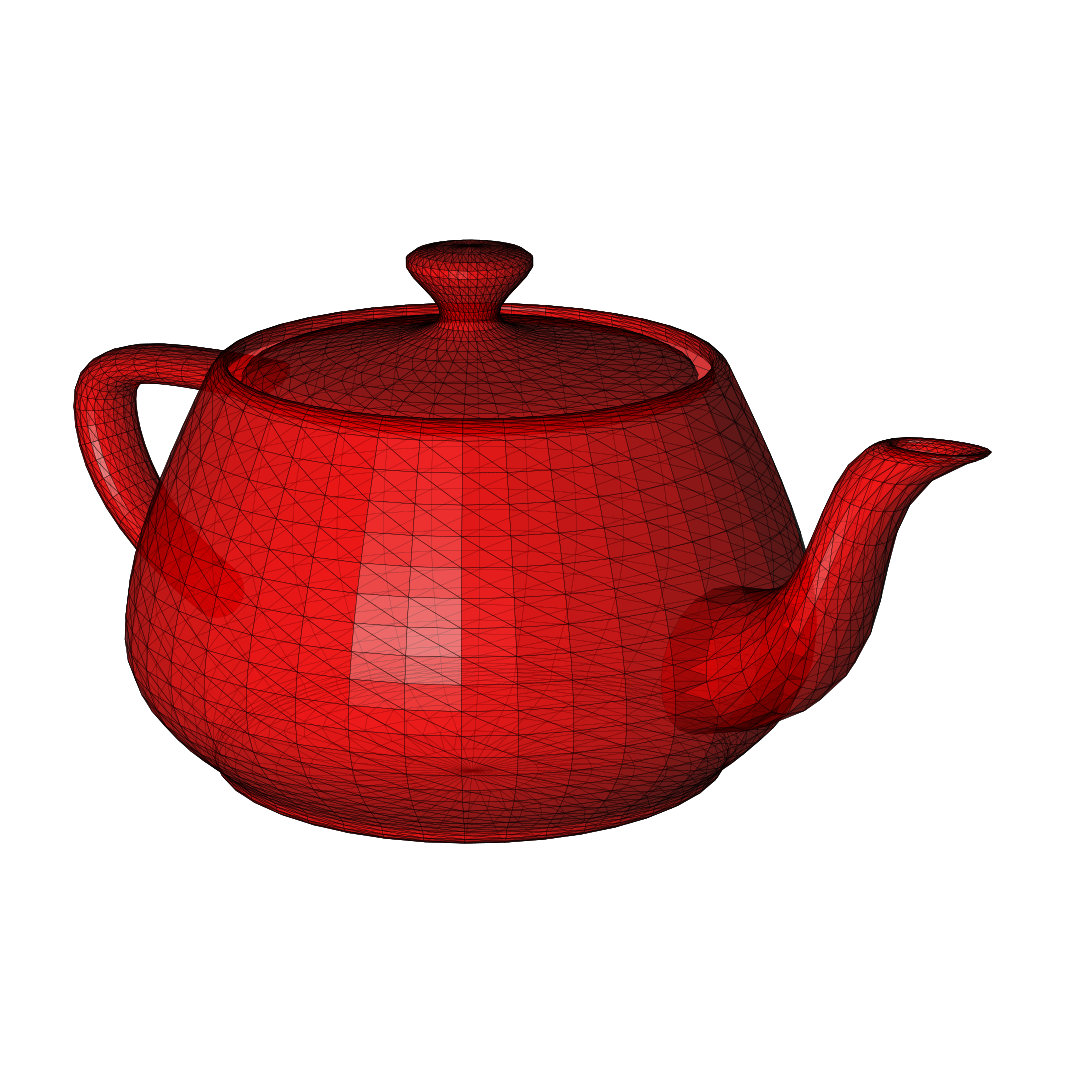
\includegraphics[scale=0.15]{img/teapot.png}
        \caption{The teapot from \texttt{examples/teapot.obj}}
        \label{fig:teapot}
    \end{figure}
    \newline\noindent The connected components can be computed using the following code
    \begin{lstlisting}
from maniflow.mesh import Mesh
from maniflow.mesh.obj import OBJFile
from maniflow.mesh.utils import connectedComponents, coincidingVertices

teapot = OBJFile.read("examples/teapot.obj")
coincidingVertices(teapot)
components = connectedComponents(teapot)

for i, component_list in enumerate(components):
    component = Mesh.fromFaceList(teapot, *component_list)
    OBJFile.write(component, "teapot" + str(i + 1) + ".obj")
    \end{lstlisting}
    \begin{figure}[ht]
    \centering
    \subfloat[The lid of the teapot]{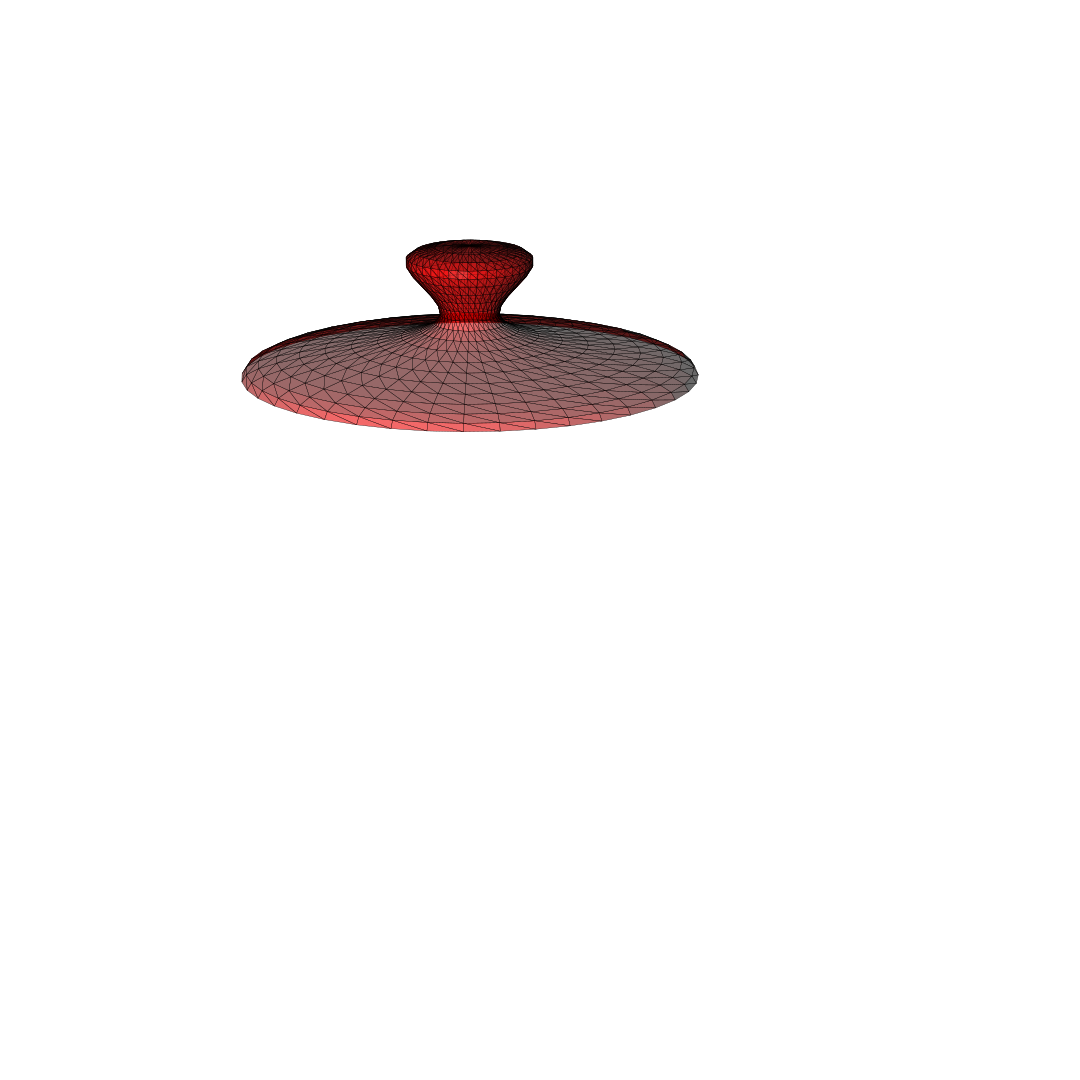
\includegraphics[width=0.4\textwidth]{img/teapot1.png}}\hfil
    \subfloat[The handle of the teapot]{
\includegraphics[width=0.4\textwidth]{img/teapot2.png}}\hfil\\
    \subfloat[The body of the teapot]{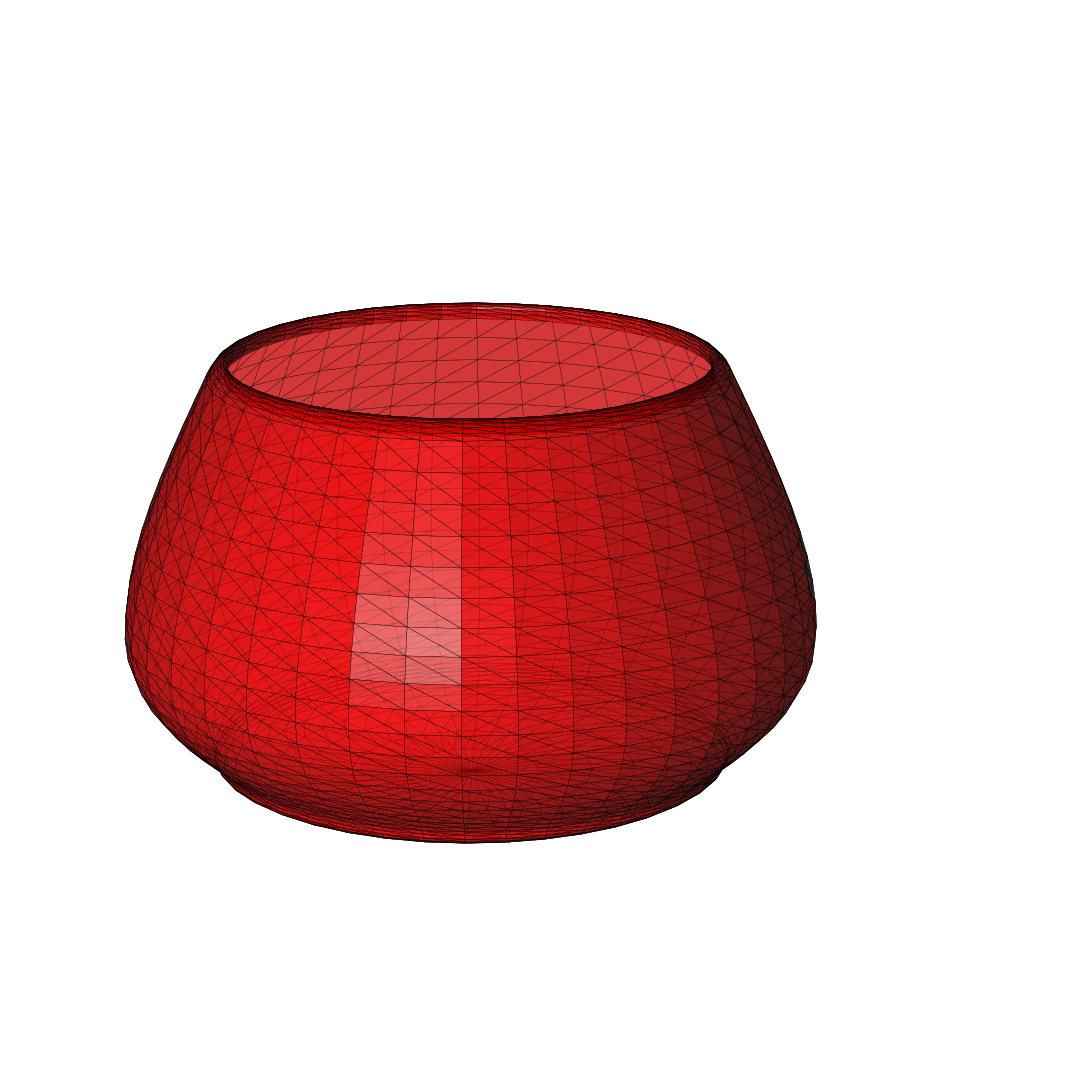
\includegraphics[width=0.4\textwidth]{img/teapot3.png}}\hfil
    \subfloat[The spout of the teapot]{
\includegraphics[width=0.4\textwidth]{img/teapot4.png}}\hfil
    \caption{The connected components of the teapot}
    \label{fig:einsteinex}
\end{figure}
\end{ex}
\end{document}

\section{Rendering meshes}
\maniflow{} employs rasterization, a fundamental technique in computer graphics, to render meshes. This process involves projecting each face of the mesh onto the viewing plane. The \texttt{maniflow.render.camera.Camera} class encapsulates the necessary matrices and operations for this projection.

\maniflow{} provides three renderers whose functionality is basically the same. Firstly, the vertices of each surface of the mesh are projected onto the display plane by means of said projections. These projected polygons (triangles) are then drawn. The only difference between the three renderers provided is how the triangles are drawn.

\subsection{The camera system}
Standard OpelGL matrices... \cite{Teschner}

\section{Geometry}
\subsection{Curvature}
\begin{ex}[Gauss-Bonnet Theorem] For a compact $2$-manifold with $\partial M = \emptyset$ we have
    \begin{align*}
        \int_M K\mathrm{d}A = 2\pi\chi(M).
    \end{align*}
    Analogously we can state a discretized version:
    \begin{align*}
        \sum_{i\in \mathrm{vert}(M)}K_i = 2\pi\chi(M).
    \end{align*}
\end{ex}
\newpage
\printbibliography
\end{document}